\chapter{Gesamtprojekt}

\section{BFMC 2023}
\autor{Felix Anslinger}
Da die \gls{BFMC} ein jährlich stattfindender Wettbewerb ist, gab es in der Vergangenheit bereits Teilnehmergruppen der Hochschule Esslingen, welche an der \gls{BFMC} teilnahmen. Zumal das Fahrzeug jedes Jahr von Bosch neu bereitgestellt wird, und nach dem Wettbewerb zurück gegeben werden muss, kann das Fahrzeug der vorherigen Teilnehmer nicht übernommen werden. 

Anders ist die Situation jedoch in Bezug auf die Software, welche auf dem Fahrzeug läuft. Es gibt diesbezüglich kein Verbot dafür, bereits existierenden Softwarestacks weiterzuentwickeln und diese als Grundlage zu verwenden. Die bei der letztjährigen \gls{BFMC} 2023 verwendete Softwarearchitektur, stellt bereits Programmcode für viele unterschiedliche Domänen eines autonomen Fahrzeugs zur Verfügung und unterteilt den Softwarestack außerdem in mehrere einzelne Komponenten. Somit folgt der Softwarestack dem \gls{SoC} Designprinzip, wodurch sich die unterschiedlichen Komponenten weitgehend unabhängig voneinander weiterentwickeln lassen (siehe Abbildung \ref{fig:softwarestack2023}). Dies ist eine maßgebende Eigenschaft des Softwarestacks und unter anderem Grund dafür, weswegen sich dieser gut als Basis für die \gls{BFMC} 2024 eignet.
\begin{figure}[H]
    \centering
    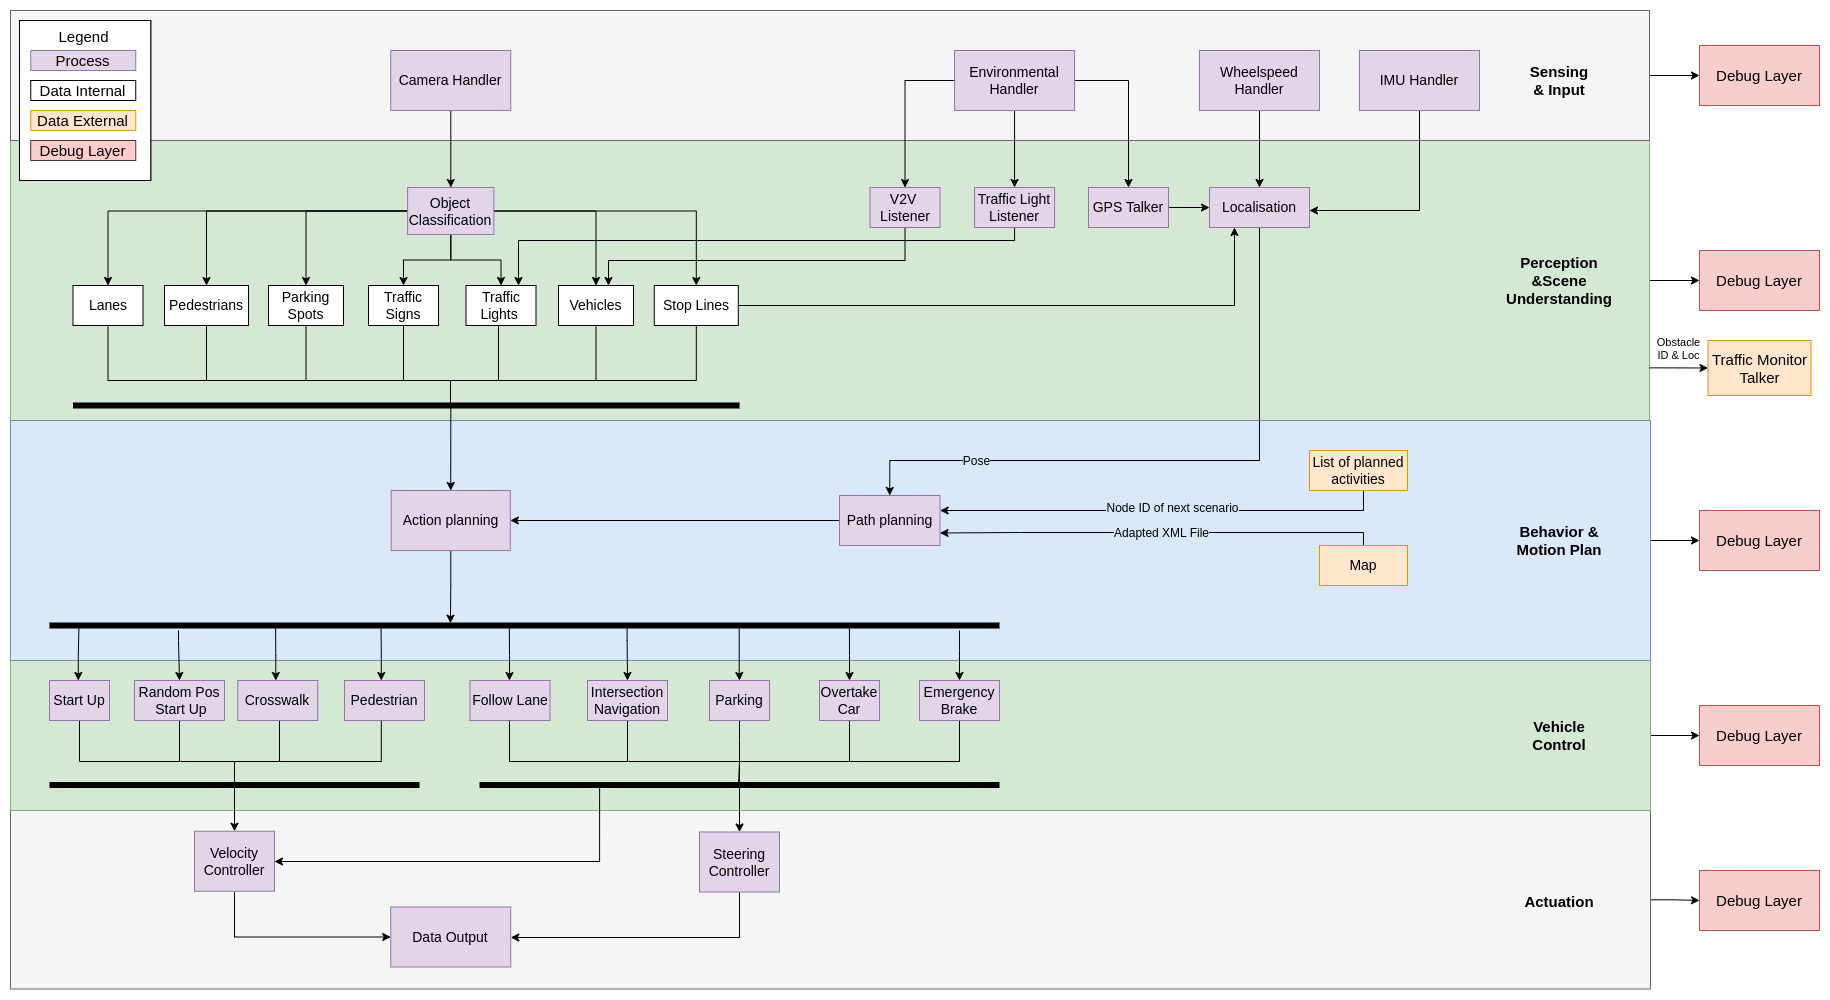
\includegraphics[width=1\linewidth]{Pictures/Project_Architecture_4_DriverlES.png}
    \caption{Softwarestack BFMC 2023}
    \cite{softwarestackBFMC2023}
    \label{fig:softwarestack2023}
\end{figure}

Die Kommunikation zwischen den einzelnen Komponenten ist durch die kollektive Implementierung von \gls{ROS} realisiert. Somit können Komponenten, wie beispielsweise die Objekterkennung, wichtige Informationen publizieren, welche dann von anderen Komponenten abgefragt und verarbeitet werden können. Durch diese Kommunikation und der Entwicklung der einzelnen Komponenten des \gls{BFMC} 2023 Softwarestacks, ist dieser bereits in der Lage, folgende Fahrsituationen zu bewältigen:
\begin{itemize}
    \item Halten der Spur
    \item Einparken
    \item Überholen von Fahrzeugen
    \item Anhalten bei Fußgängerüberwegen, Ampeln und bestimmten Verkehrsschildern
    \item Navigieren einer Kreuzung
\end{itemize}

Um diesen Softwarestack effizienter und unabhängiger von dem Fahrzeug testen zu können, wurde außerdem eine Simulationsumgebung in der Spiel-Engine Unity entwickelt (siehe Abbildung \ref{fig:unitySimulator}). Diese kann sich, anhand von \gls{ROS}, mit dem Softwarestack verbinden, wodurch simulierte Kamera-Feeds von Unity als Dateninput generiert werden können.  Die durch den Softwarestack berechneten Outputs werden dann in der Simulation umgesetzt, wodurch die Software mittels „Software in the Loop“ getestet werden kann. Dies kann im Zuge der \gls{BFMC} 2024 eingesetzt werden, um die Auswirkung von Weiterentwicklungen an dem Softwarestack in verschiedenen Fahrsituationen zu testen.

\begin{figure}[H]
    \centering
    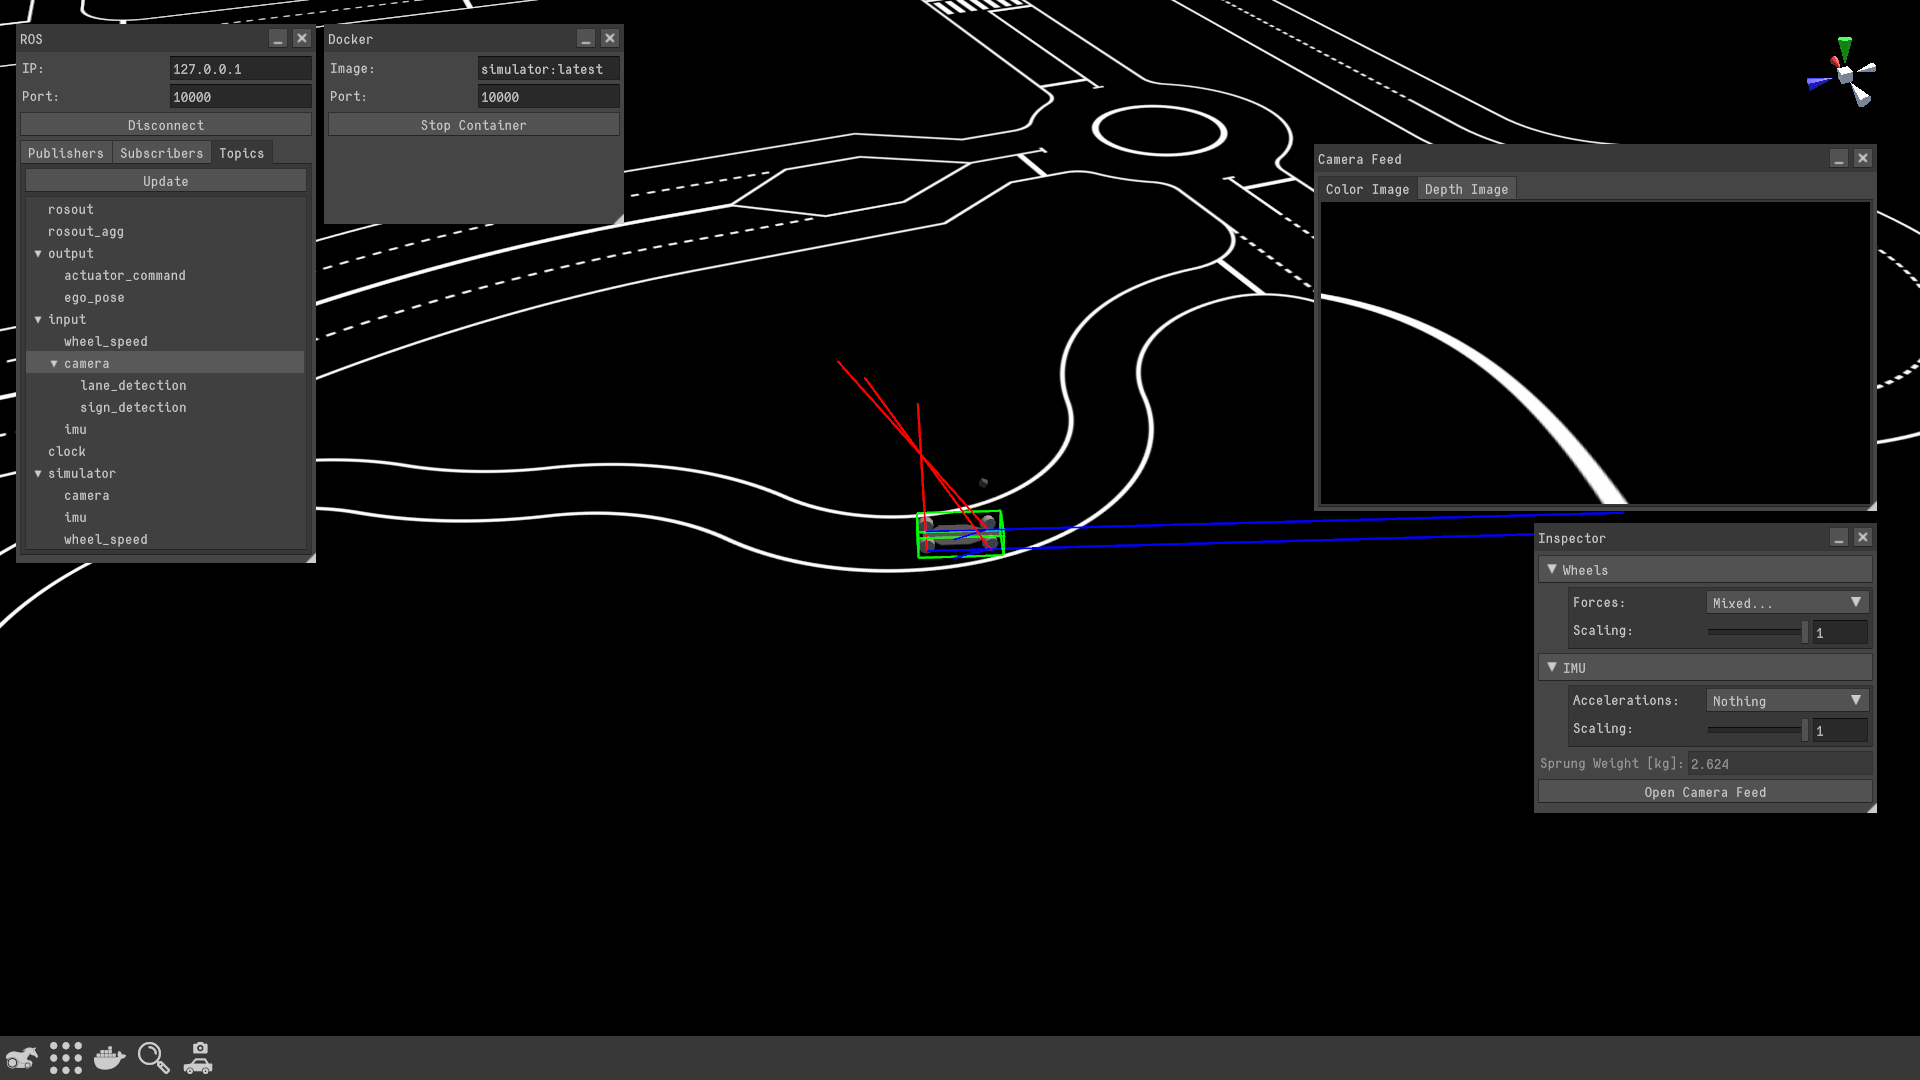
\includegraphics[width=1\linewidth]{Pictures/preview-2.png}
    \caption{Unity Simulator}
    \cite{hs_esslingen_git}
    \label{fig:unitySimulator}
\end{figure}

\newpage

\section{BFMC 2024}

\subsection{Bereitgestellte Hardware}
\autor{Felix Anslinger}

Für die \gls{BFMC} 2024 wird ein Elektro-Modellfahrzeug in dem Maßstab von 1:10 bereitgestellt. Dieses Fahrzeug besteht aus folgenden Bestandteilen: \cite{bosch_bfmc_competition_regulation}
\begin{itemize}
    \item Fahrgestell
    \item Bürstenloser Gleichstrommotor
    \item Servomotor für die Lenksteuerung
    \item \gls{IMU} für Orientierung und Geschwindigkeitsrückmeldung
    \item Mikrocontroller für Low-Level-Interaktion mit dem Fahrzeug (Nucleo F401 RE)
    \item Hauptplatine zur Entscheidungsfindung (Raspbery pi4, 8 GB)
    \item Weitwinkelkamera (Raspberry camera v3, wide)
    \item Stromverteilungsplatine zur Verwaltung der Systemleistung
    \item Batterie zur Stromversorgung
    \item Fahrzeugkarosserie zur Verdeckung der Komponenten
\end{itemize}

Diese Komponenten sind, wie in Abbildung \ref{fig:schaltplanFahrzeug} dargestellt, miteinander verbunden. 
\begin{figure}[H]
    \centering
    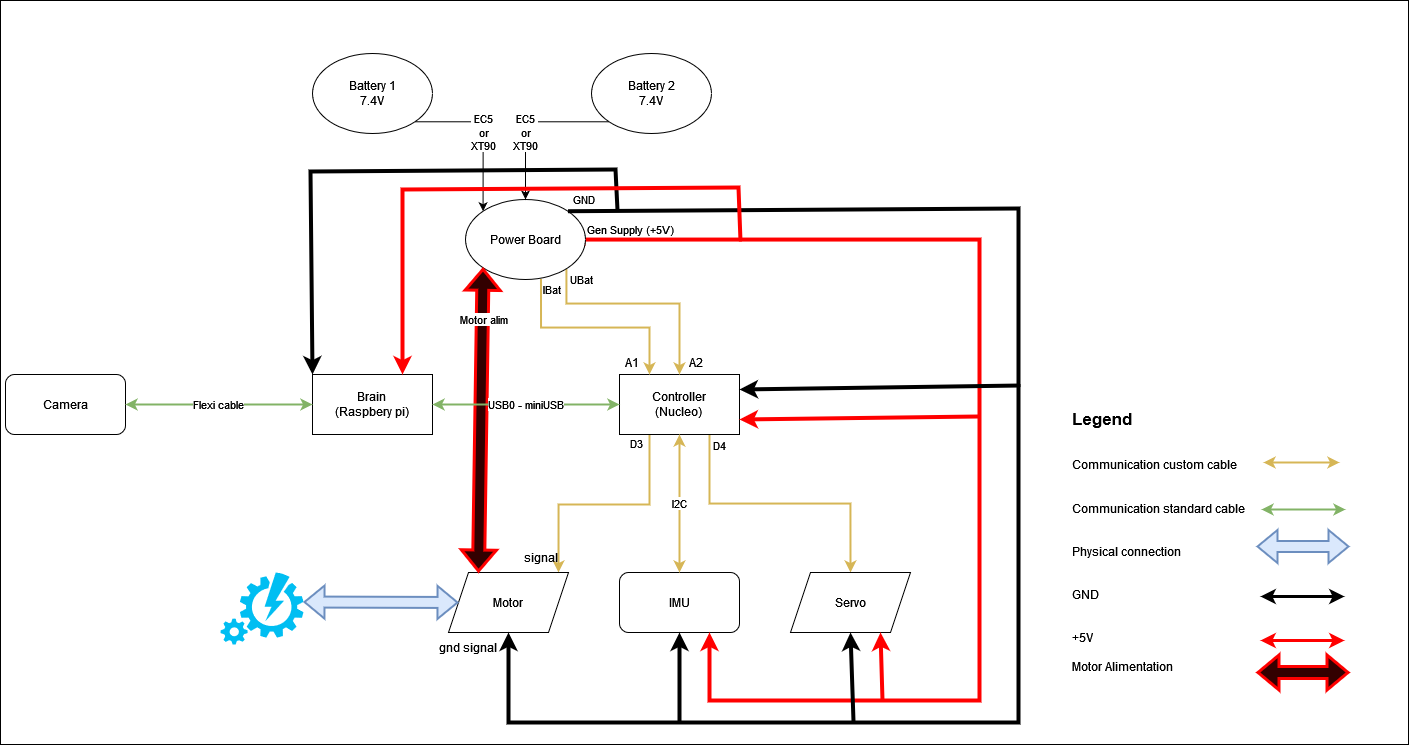
\includegraphics[width=1\linewidth]{Pictures/ConnectionDiagram.png}
    \caption{Schaltplan der Hardware des Fahrzeuges}
    \cite{bosch_bfmc_competition_documentation}
    \label{fig:schaltplanFahrzeug}
\end{figure}

\newpage
\subsection{Hardware Upgrades}
\autor{Gamze Isik, Aaron Müller}

Für die Ausstattung der Hardware wird der NVIDIA Jetson Orin NX \cite{jetson-orinNX} in Verbindung mit dem Carrierboard JETSON ORIN IO \cite{jetson-orinIO} sowie dem Reflection Sensor QTR-1A\cite{reflection-sensor} verwendet, um das Fahrzeug entsprechend zu modifizieren. Der Einsatz des NVIDIA Jetson Orin NX erweist sich als vorteilhafter im Vergleich zum Raspberry Pi mit 8GB, da der Jetson Orin NX eine höhere Leistungsfähigkeit besitzt. Dieser übernimmt die Funktion des Gehirns und führt Berechnungen durch, während \gls{ROS} ausgeführt wird. 
Die höhere Leistung ist besonders auch für KI-Algorithmen notwendig, wie z.B. einer Semantischen Segmentierung oder Objekterkennung.\\

Die Reflection Sensoren werden oft in Robotik- und Elektronikprojekten eingesetzt, um Linienverfolgungsaufgaben oder die Erkennung von Oberflächen zu ermöglichen. Im Kontext des zuvor genannten Textes wird der QTR-1A Reflectance Sensor verwendet, um die gefahrene Distanz und die Geschwindigkeit des Fahrzeugs zu messen, indem er die reflektierte Infrarotstrahlung von Markierungen auf den Rädern erfasst.\\

Auf die Anschaffung einer neuen Kamera verzichtet, stattdessen wird die mitgelieferte Raspberry Pi Kamera genutzt.
Alternativ wäre es möglich gewesen, eine Stereokamera wie z.B. die Intel Realsense\cite{intel-realsense} zu verwenden, welche zusätzlich zu den Bilddaten Tiefeninformationen liefert.
Das von den Regularien vorgeschriebene Budget reicht jedoch nicht für die zusätzliche Verwendung der teuren Kamera, sodass Abstände von Objekten auf dem Bild errechnet werden müssen.
Sollte sich die Berechnung schwieriger gestalten als gedacht, können auch günstige Ultraschall- oder LiDAR-Sensoren verwendet werden.

\newpage
\subsection{Regularien}
\autor{Gamze Isik}

Die Regularien für die \gls{BFMC} 2024 unterscheiden sich von denen des letzten Jahres. Die Rennstrecke weist eine andere Route im Vergleich zum Vorjahr auf. Die Strecke umfasst verschiedene Straßenelemente, darunter:

\begin{itemize}
    \item Gerade Streckenabschnitte
    \item Kurven
    \item Kreuzungen (mit 3 oder 4 Straßenbegegnungen)
    \item Parallelparkplätze
    \item Einspurige Straßen
    \item Zweispurige Straßen
    \item Autobahnen
    \item Kreisverkehre
    \item Einbahnstraßen
    \item Rampen
\end{itemize}

\begin{figure}[!h]
    \centering
    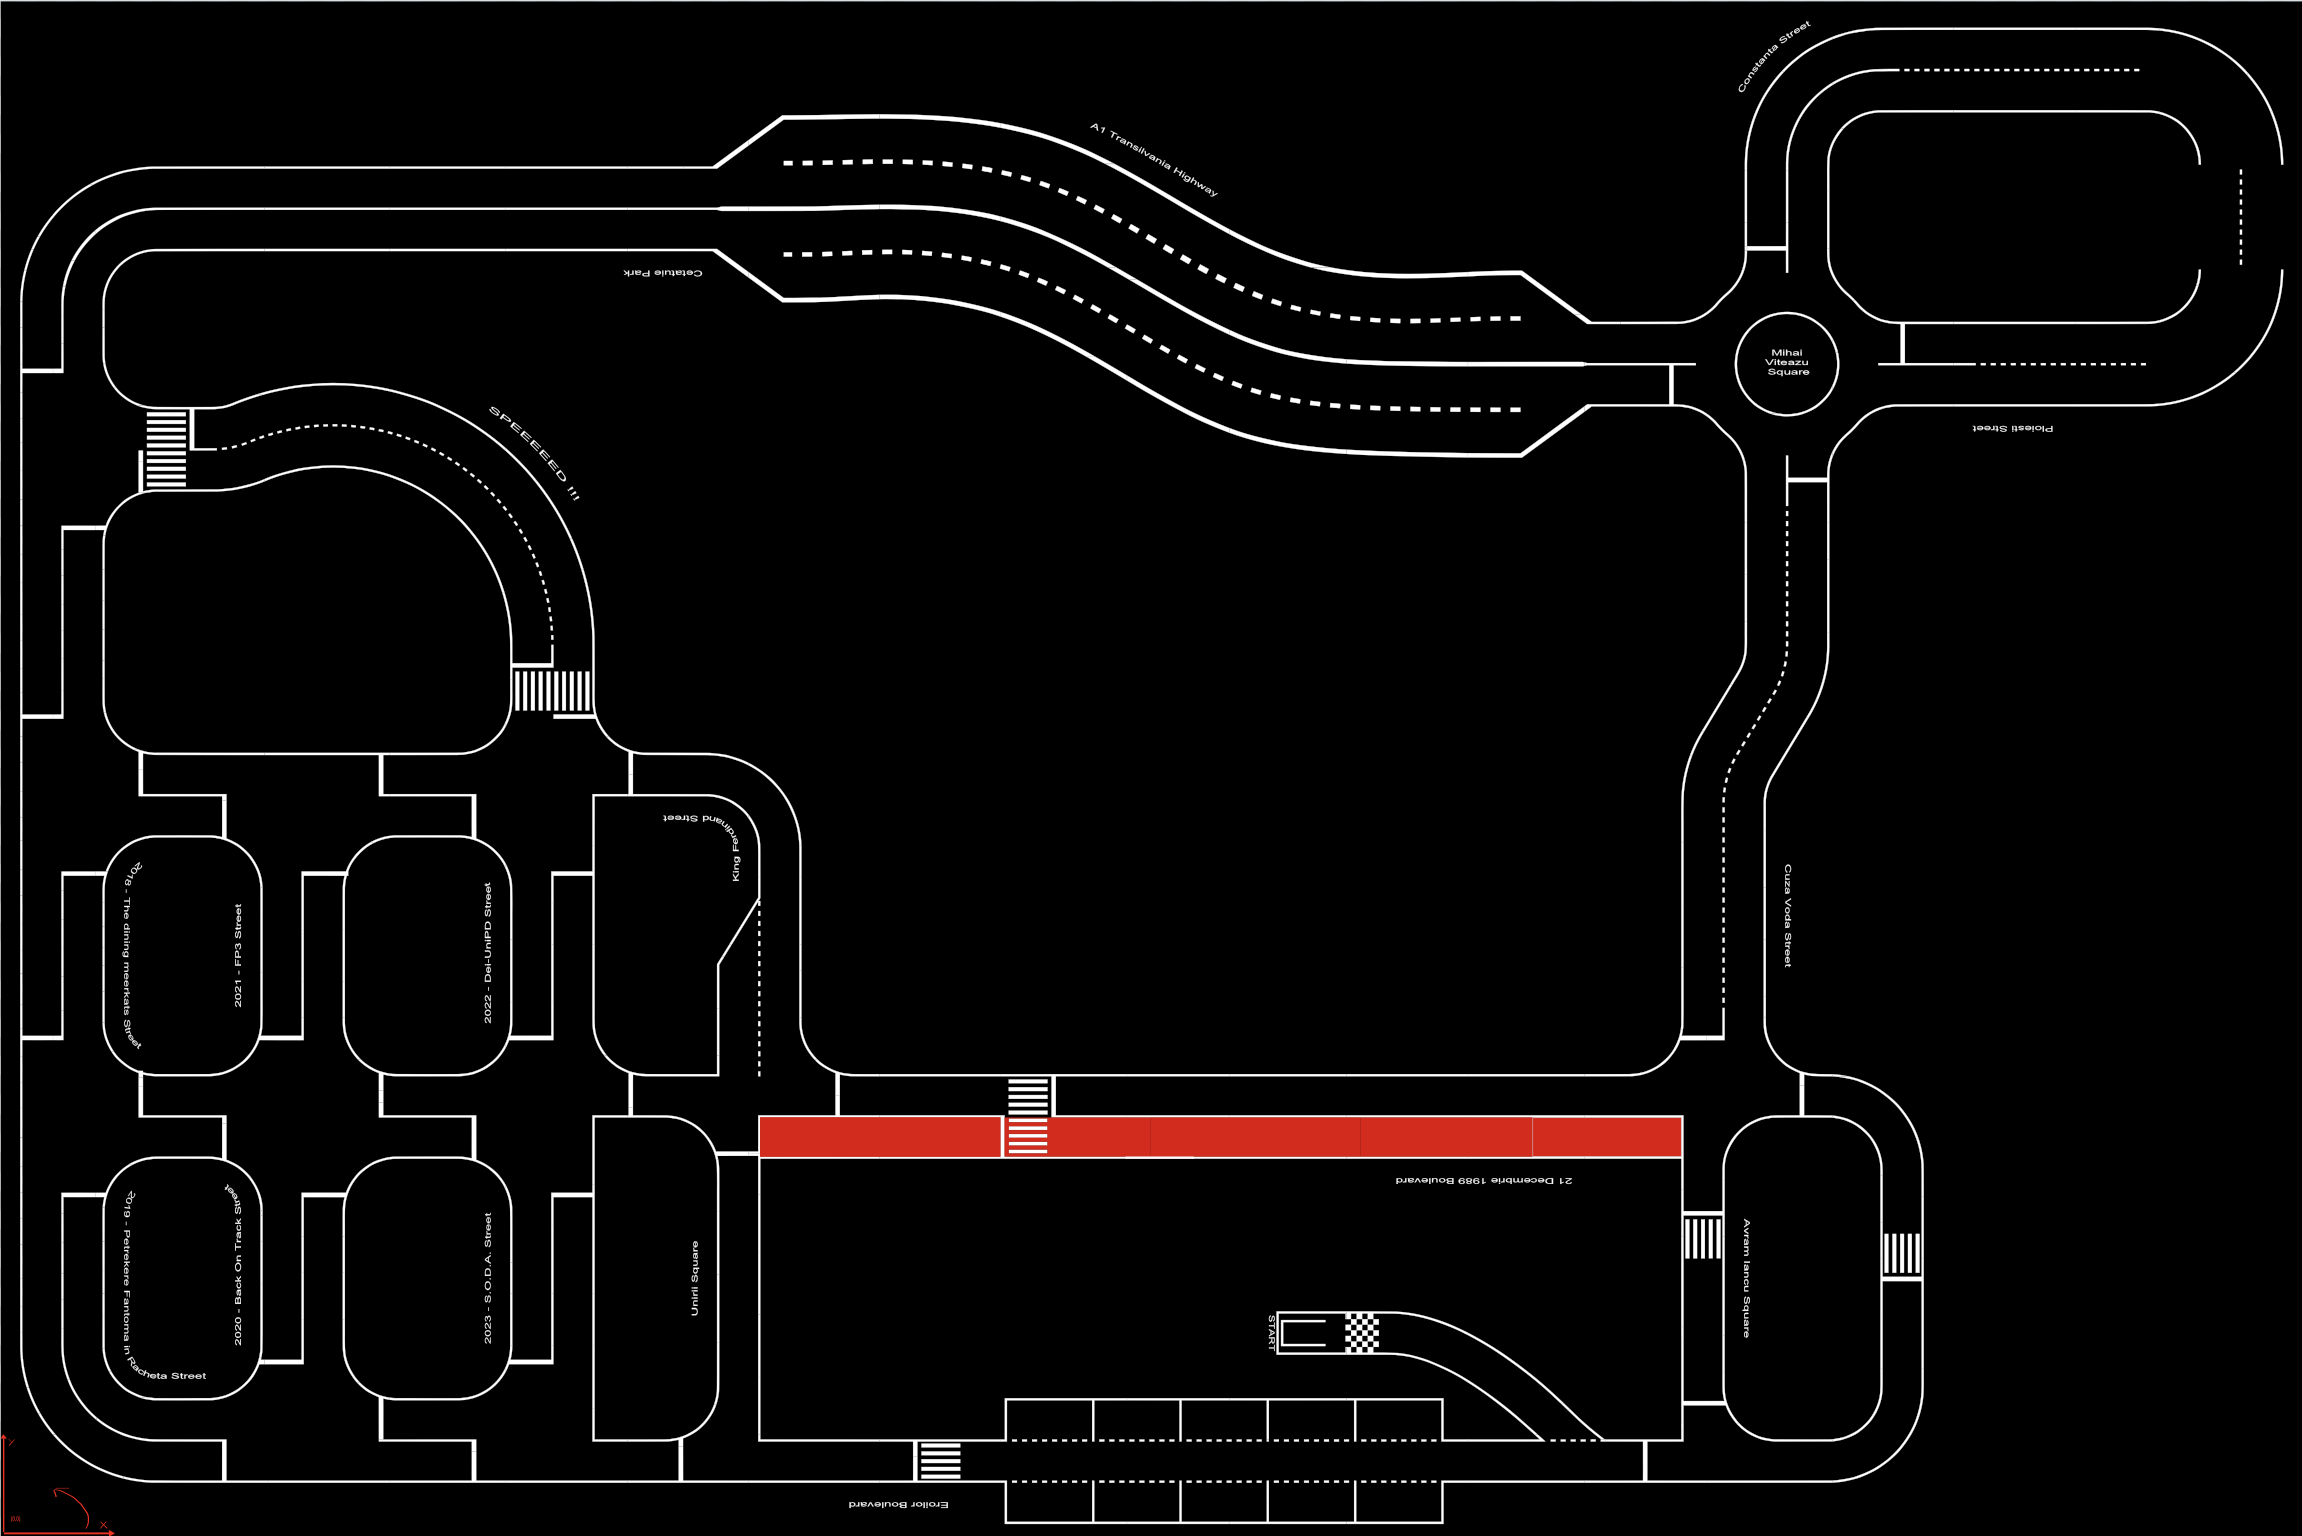
\includegraphics[width=1\linewidth]{Pictures/RaceTrack.png}
    \caption{\gls{BFMC} 2024 Race Track}
    \label{fig:race-track}
\end{figure}

\newpage

Die Fahrspurbreiten auf der rechten und linken Seite betragen jeweils etwa 35 cm, während die weißen Fahrspurlinien 2 cm breit sind (sofern nicht anders angegeben).\cite{bfmc-roadMark}

\begin{figure}[!h]
    \centering
    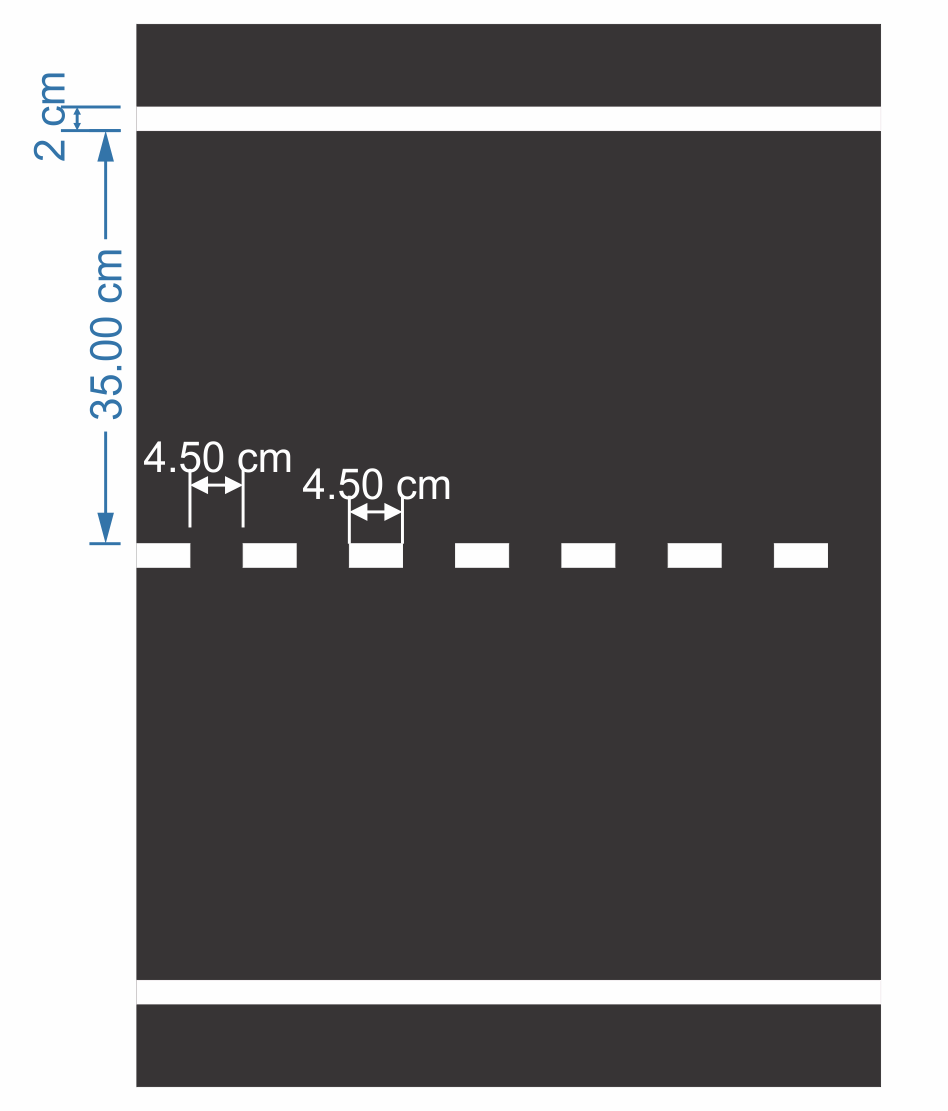
\includegraphics[width=0.5\linewidth]{Pictures/road.png}
    \caption{Straßen Bemessung}
    \cite{bfmc-roadMark}
\end{figure}

Des Weiteren werden Verkehrsregeln aufgestellt, die in der Tabelle \ref{traficRules} aufgelistet sind.\\

Die \gls{BFMC} stellt eine Reihe von Systemen bereit, die sich mit dem Aspekt der Konnektivität in der Herausforderung befassen. Diese Systeme replizieren die Umgebung einer intelligenten Stadt und bieten den Teilnehmern vielfältige Möglichkeiten zur Entwicklung ihrer Projekte. Dadurch können sie Daten fusionieren und validieren sowie geteilte Daten anfordern und senden. Die verfügbaren Systeme sind:

\begin{itemize}
    \item Ein Lokalisierungssystem
    \item Ein Echtzeit-Verkehrsüberwachungssystem
    \item Intelligente Ampeln
    \item Fahrzeugkommunikation
\end{itemize}

\textbf{Lokalisierungssystem}\\

Es handelt sich um eine physische Box, die während der Fahrt auf dem Auto platziert wird. Es bietet die ungefähre Position des Fahrzeugs auf der Strecke mit einer Frequenz von etwa 5 Hz. Das System hat einen maximalen Fehlerradius von 20 cm und eine Verzögerung von bis zu 0,5 Sekunden.\cite{bfmc-vehicle2everyth}\\
\newpage
\textbf{Verkehrskommunikationssystem}\\

Jedes Auto muss Daten an ein hauseigenes Verkehrskommunikationssystem senden, darunter die Arten von Hindernissen (basierend auf Ereignissen), Fahrzeuggeschwindigkeit, Fahrzeugposition und Fahrzeugausrichtung, einmal alle 3 Sekunden (oder weniger). Die Daten werden verwendet, um die Details der gerade durchgeführten Fahrt des Autos nachzubilden.\cite{bfmc-vehicle2everyth}\\

\textbf{Intelligente Ampel}\\

Die Ampeln teilen ihren Status im Netzwerk mit, indem sie ihren Farbzustand und ihre Position auf der Karte anzeigen. Die Frequenz der gesendeten Nachrichten beträgt 1 Hz.\cite{bfmc-vehicle2everyth}\\

\textbf{Fahrzeugkommunikation}\\

Fahrende Fahrzeuge übermitteln ihre Positionen im Netzwerk mithilfe von Rohwerten aus dem Lokalisierungssystem. Die Frequenz der gesendeten Nachrichten beträgt 5 Hz, wobei Genauigkeit und Verzögerung direkt mit dem GPS korreliert sind.\cite{bfmc-vehicle2everyth}

\subsubsection{Technische Herausforderung}\\

\quote{In der technischen Herausforderung startet das Fahrzeug des Teams von einem festgelegten Punkt (entweder der START-Position oder der zufälligen Position, die vom Jury ausgewählt wurde, wenn das Hindernis gewählt wurde).\\
Ab diesem Zeitpunkt ist nur der Einsatz eines Dashboards als Computer und laufende Software erlaubt, das als Teil des Startcodes bereitgestellt wird (die Verwendung anderer Steuerungen, Geräte oder Anwendungen ist verboten). Die App dient als Überwachungsanwendung, in der das teilnehmende Team, das Organisations- und Jury-Team oder andere Teilnehmer in Echtzeit den Zustand des Fahrzeugs überprüfen können. Jedes Team kann sein Dashboard an seine eigenen Bedürfnisse anpassen oder es von Grund auf neu erstellen. Die technische Herausforderung sollte direkt von der App aus gestartet werden. Ein Verkehrslicht mit rotem Licht wird am Startpunkt vorhanden sein. Die Jury gibt das Startsignal durch Drücken ihres eigenen Startknopfes und Ändern der Farbe des Verkehrslichts von Rot auf Grün. Das Fahrzeug muss den Start der Fahrt autonom erkennen und den spezifischen Szenarien (beschrieben im Abschnitt zur Punktevergabe) des Teams folgen.\\
Teams können ihre optionalen Szenarien für zusätzliche Punkte auswählen, solange die Laufzeit eingehalten wird (Die Fahrt selbst wird bei Erreichen des 10-Minuten-Limits gestoppt). Szenarien können in beliebiger Reihenfolge angegangen werden, aber Teams müssen die Organisatoren über die ausgewählten optionalen Herausforderungen informieren und möglicherweise den Pfad ihres Fahrzeugs mitteilen (falls der zufällige Startpunkt nicht ausgewählt wurde).} \cite{bfmc-competition}